In questo capitolo parler\`o dell'algoritmo utilizzato durante la fase di sperimentazione.

Tutti i PoS tagger esistenti, considerano la parola, o pi\`u generalmente il
\emph{token}, come l'unit\`a fondamentale dell'apprendimento. Molti algoritmi
prevedono delle fasi di preprocessing del testo atte a semplificarlo, eliminando
molte delle varianti tipiche di una lingua naturale, come ad esempio la \emph{lemmatizzazione}.

La lemmatizzazione consiste nel ridurre una forma \emph{flessa}\footnote{In
linguistica si chiama \emph{flessione} una qualsiasi variazione morfologica delle
parole realizzata per indicarne i tratti grammaticali o sintattici. Avremo ad
esempio diverse forme flesse di un verbo (\emph{io lavoro}, \emph{tu lavori})
oppure di un nome (\emph{il lavoro}, \emph{i lavori}).} di una parola alla sua
forma canonica (non marcata), detta \emph{lemma}\footnote{In linguistica si dice
lemma la citazione di una parola, ossia quella parola che per convenzione è scelta
per rappresentare tutte le forme di una flessione.}. Esistono numerosi algoritmi
di lemmatizzazione come, ad esempio, \emph{Lovins}~\cite{Lovins:1968} e
\emph{Porter}~\cite{Porter:1980}. Entrambi sono algoritmi di \emph{suffix stripping}
che rimuovono, quindi, i suffissi alle parole a partire da un dizionario di suffissi
comuni.

Altro problema \`e la tokenizzazione, ossia la suddivisione del testo in token.
Processo che all'apparenza sembra di semplice soluzione ma che nasconde delle
difficolt\`a. Prendiamo in considerazione \texttt{aren't}, qual \`e la tokenizzazione
corretta? Possiamo infatti avere \texttt{aren't}, \texttt{arent}, \texttt{are nt}
e \texttt{aren t}.

I dizionari poi, vengono costruiti a partire alle parole presenti nel corpus.
La fase di preprocessing \`e fondamentale nella costruzione di un dizionario
efficiente, altrimenti si avrebbero dizionari enormi con un elevato numero di
parole che, pur avendo quasi lo stesso significato (es. \emph{lavoro}, \emph{lavori})
sono rappresentati in maniera del tutto differente e senza alcuna correlazione.

In questa tesi si cercher\`a di cambiare approccio. L'unit\`a base sar\`a il
singolo carattere, piuttosto che il token. Questo approccio semplifica di molto
la fase di preprocessing del testo, eliminandola del tutto. Non sar\`a pi\`u
necessario ne tokenizzare ne lemmatizzare il corpus in input.

\section{Algoritmo per POS-Tagging basato su caratteri}

La totalit\`a dei corpus taggati, nonch\`e dei tagset esistenti, prevedono dei tag
per le parole e non per i caratteri. Quindi, il primo passo per poter addestrare
con successo un PoS-Tagger basato su caratteri, consiste nel trasformare i dataset
scelti.

La trasformazione \`e stata effettuata in questo modo:
\begin{itemize}
  \item Ogni parola del dataset \`e stata divisa in caratteri.
  \item Ad ogni carattere cos\`i ottenuto, \`e stata assegnata la classe della
        parola di appartenenza.
  \item Alle classi assegnate a ciascun carattere sono stati aggiunti dei suffissi:
  \begin{itemize}
    \item il suffisso \emph{-S} (\emph{S}tart) alla classe del primo carattere
          di ogni parola.
    \item il suffisso \emph{-I} (\emph{I}nner) alla classe degli altri caratteri
          della parola.
  \end{itemize}
\end{itemize}

Ad esempio:

\begin{center}
  \begin{minipage}{5cm}
    \begin{verbatim}
     .
     .
     reckons   VBZ
     .
     .
    \end{verbatim}
  \end{minipage}
\end{center}

diventa

\begin{center}
  \begin{minipage}{5cm}
    \begin{verbatim}
     .
     .
     r   VBZ-S
     e   VBZ-I
     c   VBZ-I
     k   VBZ-I
     o   VBZ-I
     n   VBZ-I
     s   VBZ-I
     .
     .
    \end{verbatim}
  \end{minipage}
\end{center}

Un possibile problema nell'addestrare un PoS-Tagger basato su caratteri, riguarda
la separazione fra le parole. Nel PoS-Tagging tradizionale la separazione fra le
parole \`e implicita, ogni token corrisponde ad una parola. Nel nostro caso, non
essendoci alcun tipo di tokenizzazione, si rischia di perdere un'informazione
importante, ossia dove termina una parola e ne inizia un'altra. Una possibile
soluzione consiste nell'aggiungere, in fase di trasformazione del dataset, un
carattere di spazio fra i caratteri delle singole parole ed assegnare a questo
carattere il tag speciale \emph{S}. Tuttavia, questa soluzione, potrebbe non essere
strettamente necessaria. La rete, infatti, potrebbe apprendere lo stesso questa
informazione, grazie al suffisso dato ai tag (-S indica implicitamente l'inizio
di una parola). Difficile determinare a priori quale sia la scelta migliore,
pertanto si \`e optato per adottarle entrambe addestrando pi\`u reti, met\`a
delle quali addestrate con l'aggiungere il carattere di spazio e l'altra met\`a
senza.

Il passo successivo \`e stato quello di creare due dizionari, uno per i caratteri e
l'altro per i tag. Entrambi i dizionari consistono in un insieme di coppie \texttt{
chiave => valore }, dove il \texttt{vaolre} \`e, in entrambi i dizionari, un numero
intero univoco. La \texttt{chiave}, invece, \`e costituita dal carattere, per
quanto riguarda il dizionario dei caratteri, e dal tag, per quanto riguarda il
dizionario dei tag.

Con i dataset convertiti in una sequenza di caratteri e i dizionari per carattere
e tag, \`e possibile iniziare ad addestrare una rete neurale LSTM descritto nell'
algoritmo seguente (algoritmo~\ref{alg:train}).


\begin{algorithm}[ph] \label{alg:train}
  \SetKwFunction{LSTM}{LSTM}\SetKwFunction{size}{size}
  \SetKwFunction{onehot}{onehot}\SetKwFunction{ClassNLLCriterion}{ClassNLLCriterion}
  \SetKwInOut{Input}{input}\SetKwInOut{Output}{output}

  \Input{il training set $\mathcal{D}$, il dizionario $\mathcal{C}$ dei caratteri,
  il dizionario $\mathcal{T}$ dei tag, epoca massima $\varepsilon$, numero di nodi $j$, numero
  di livelli $l$}
  \Output{l'insieme $\mathcal{W}$ dei pesi della rete addestrata}
  \BlankLine
  \tcc{creo la rete neurale LSTM specificando n. di nodi in input, numero di nodi
  in output, numero di livelli nascosti e numero di nodi per livello nascosto}
  $model \gets $ \LSTM{\size{$\mathcal{C}$}, \size{$\mathcal{T}$},
  $l$, $j$}

  \tcc{la funzione di perdita per problemi di classificazione}
  $criterion \gets $ \ClassNLLCriterion{}

  \For{$i \gets 1$ \textbf{to} $\varepsilon$} {
    \For{$char, tag \in \mathcal{D}$} {
      \tcc{codifica onehot per carattere e tag}
      $x \gets $ \onehot{$\mathcal{C}[char]$}

      $y \gets $ \onehot{$\mathcal{T}[tag]$}

      $prediction \gets model.forward(x)$

      $error \gets criterion.forward(prediction, y)$

      $gradOutputs \gets criterion.backward(error, y)$

      $model.backward(x, gradOutputs)$
    }
  }

  $\mathcal{W} \gets model.weights$

  \tcc{restituisco i pesi della rete neurale.}
\caption{$Addestramento$}
\end{algorithm}

\section{Codifica One-Hot}
Dall'algoritmo si possono notare, in particolare, due aspetti che, a dispetto di
quanto si possa immaginare, sono strettamente collegati:

\begin{itemize}
  \item Il numero di nodi in input e output, per la creazione di una rete LSTM,
        sono, rispettivamente, la dimensione del dizionario $\mathcal{C}$ dei
        caratteri e la dimensione del dizionario $\mathcal{T}$ dei tag
  \item Ogni carattere e ogni tag del dataset \`e stato codificato, prima di essere
        dato in input alla rete neurale, con una codifica \emph{One Hot}.
\end{itemize}

Nella codifica One Hot, ad ogni dato che vogliamo rappresentare, \`e associato
un vettore di $n$ bit. La dimensione di $n$ dipende dal numero di dati differenti
che vogliamo poter rappresentare. Infatti, di questi $n$ bit, solo uno \`e acceso
(1) mentre tutti gli altri sono spenti (0). \`E evidente, quindi, che con $n$ bit
\`e possibile rappresentare al massimo $n$ informazioni diverse.

Prendiamo, ad esempio, la codifica in One Hot dei caratteri presenti nel nostro
dataset. In questo caso, il numero massimo di valori rappresentabili \`e dato
dalla dimensione del dizionario dei tag, quindi $n = \operatorname{length}
(\mathcal{C})$. Supponiamo, per semplicit\`a, di avere solo 4 caratteri nel nostro
dizionario (\ref{eq:dictag}).

\begin{equation} \label{eq:dictag}
  \mathcal{C} = \{ ``a", ``b", ``c", ``d" \}
\end{equation}

Ogni carattere sar\`a quindi rappresentato con un vettore di 4 bit in questo modo:

\begin{equation}
  \vec{a} = [ 1, 0, 0, 0]
\end{equation}
\begin{equation}
  \vec{b} = [ 0, 1, 0, 0]
\end{equation}
\begin{equation}
  \vec{c} = [ 0, 0, 1, 0]
\end{equation}
\begin{equation}
  \vec{d} = [ 0, 0, 0, 1]
\end{equation}

Il numero di nodi di input e output \`e diretta conseguenza della scelta di usare
questa codifica. Infatti, per poter dare in input alla rete vettore $\vec{b}$, ad
esempio, sono necessari 4 nodi di input (Figura~\ref{fig:nnInputExample}).

\begin{figure}[tp]
  \centering
  \begin{center}
    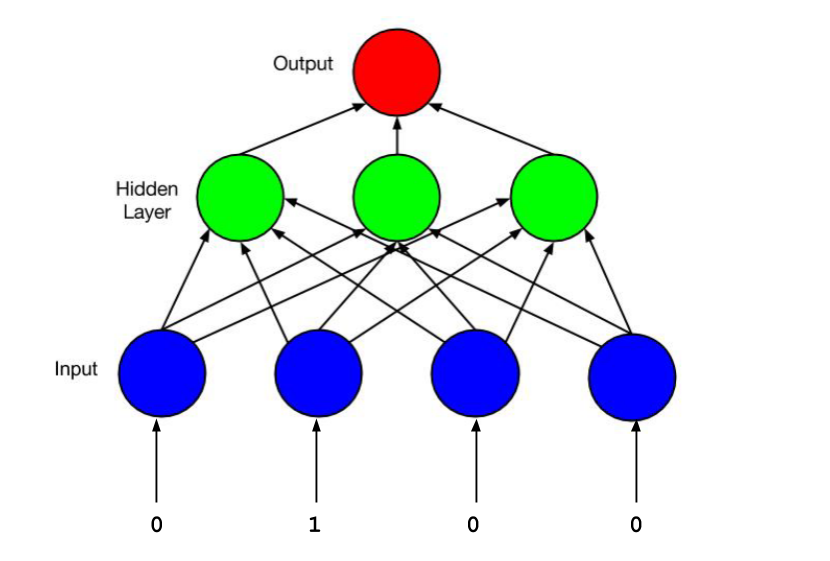
\includegraphics[width=0.7\textwidth]{./images/nnInputExample.png}
  \end{center}
  \caption{il vettore $\vec{b} = [ 0, 1, 0, 0]$ dato in input ad una rete neurale
  con 4 nodi di input}
  \label{fig:nnInputExample}
\end{figure}

In output la rete deve restituire a, sua volta, un tag codificato con codifica
One Hot. Di conseguenza, il numero dei nodi di output \`e dato dal numero di tag
possibili.

Dall'algoritmo proposto si evince, dunque, che il numero di nodi di input \`e pari
al numero di caratteri presenti nel dizionario $\mathcal{C}$ dei caratteri e,
allo stesso modo, il numero dei nodi di output \`e pari al numero di tag nel
dizionario $\mathcal{T}$ dei tag.


\section{Valutazioni}

Dal training set \`e stato estratto un piccolo insieme (\~10\% del training set)
usato come validation set durante tutta la fase di addestramento per monitorarne
l'andamento, calcolando periodicamente, su questo insieme di dati, il \emph{loss}
(il valore dell'errore calcolato dalla funzione di perdita).

Per ogni dataset sono state addestrate 96 reti LSTM, ciascuna delle quali
differisce dalle altre per:

\begin{itemize}
  \item numero di livelli (2, 3, 4, 5)
  \item numero di nodi (128, 256, 512, 1024)
  \item numero di fasi temporali (60, 80, 100)
  \item uso o meno del carattere di spazio
\end{itemize}

Ogni rete neurale \`e stata addestrata fino alla 150\textsuperscript{$\circ$} epoca.

A queste reti \`e stato poi dato in input il test set, un carattere alla volta,
utilizzando lo stesso dizionario calcolato durante la fase di addestramento e con
codifica One Hot.

La rete ha quindi classificato singolarmente tutti i caratteri del test set,
dando a questi utlimi una classe col suffisso \emph{-S} e \emph{-I}. L'output
dato dalla rete per ciascun carattere consiste in un vettore di probabilit\`a.
Ciascun elemento del vettore corrisponde ad una determinata classe, e il valore
dell'elemento corrisponde alla probabilit\`a che quella determinata classe sia la
classe corretta per quel carattere. A partire da questo vettore \`e stata quindi
seleziona la classe corrispondente alla probabilit\`a pi\`u alta. Una volta ottenute
le classi di ciascun carattere, \`e stata estratta la classe della parola di appartenenza
di ogni carattere scegliendola fra la classe di maggioranza dei singoli caratteri.

Ad esempio, i caratteri della parola \texttt{reckons} sono stati classificati
dalla rete neurale in questo modo:

\begin{center}
  \begin{minipage}{5cm}
    \begin{verbatim}
     .
     r   VBZ-S
     e   PRP-I
     c   VBZ-I
     k   VBZ-I
     o   NN-I
     n   VBZ-I
     s   VBD-I
     .
     .
    \end{verbatim}
  \end{minipage}
\end{center}

La classe che si ripete con pi\`u frequenza in questa sequenza di caratteri, a
meno del suffisso, \`e \texttt{VBZ}, di conseguenza l'intera parola \texttt{reckons}
\`e stata classificata come

\begin{center}
  \begin{minipage}{5cm}
    \begin{verbatim}
     reckons   VBZ
    \end{verbatim}
  \end{minipage}
\end{center}
